\section{Geometría Proyectiva}
\subsection{Contexto e idea}
Segun el programa de Erlegen, una geometría se basa en el estudio de invariantes
al aplicar unas ciertas transformaciones. Así tenemos que las geometrías estan
"incluidas" en las superiores.

Así, la geometría euclidea, que estudia las transformaciones ortogonales, estaría
"incluída" en la geometría afín, que estudia las tansformaciones lineales. Aquí
se muestra una tabla con las distintas geometrías en la cual cada una esta
"incluída" en la anterior
\begin{center}
	\begin{tabular}{|c|c|}
		\hline Geometría & Transformaciones de estudio \\
		\hline \hline
		G. euclídea  & transformaciones ortogonales \\ \hline
		G. afín & transformaciones lineales \\ \hline
		G. proyectiva & proyectividades \\ \hline
		G. Algebraica & transformaciones por polinomios \\ \hline
		G. Analítica & transformaciones por funciones analíticas \\ \hline
		G. Diferencial & transformaciones por funciones de clase
		$\mathcal{C}^\infty$ \\ \hline
		Topología & transformaciones por funciones de clase $\mathcal{C}^0$\\ \hline
	\end{tabular}
\end{center}

\subsubsection{Problema matemático}
\begin{center}
	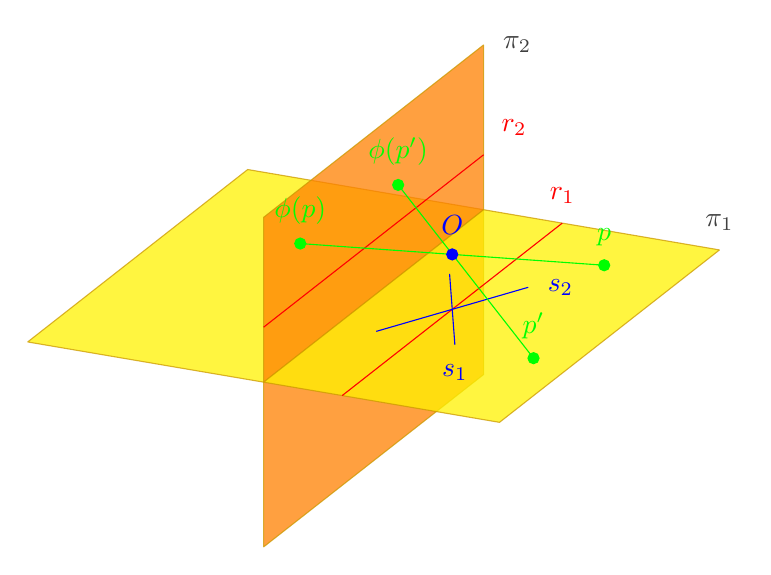
\begin{tikzpicture}
	\begin{axis}[%
	hide axis,
	width=\columnwidth,
	enlargelimits=0.1
	]
	
	\addplot3[patch, patch type=rectangle,opacity=.75,color=yellow]
	coordinates {(0,3,0) (-3,3,0) (-3,-3,0) (0,-3,0)};
	\addplot3[patch, patch type=rectangle,opacity=.75,color=orange]
	coordinates {(0,3,-3) (0,-3,-3) (0,-3,3) (0,3,3)}
	node[label={[black]right:$\pi_2$}]{};
	\addplot3[patch, patch type=rectangle,opacity=.75,color=yellow]
	coordinates {(3,-3,0) (0,-3,0) (0,3,0) (3,3,0)}
	node[label={[black]$\pi_1$}]{};
	
	\addplot3[color=blue,mark=*] coordinates {(1,0,1)}
	node[label=above:{$O$}]{};
	
	\draw [color=red] (axis cs:1,-3,0) -- (axis cs:1,3,0)
	node[label=$r_1$]{};
	\draw [color=red] (axis cs:0,-3,1) -- (axis cs:0,3,1)
	node[label=50:$r_2$]{};
	
	\draw [color=blue] (axis cs:0.5,1,0) -- (axis cs:1.5,-1,0)
	node[label=below:$s_1$]{};
	\draw [color=blue] (axis cs:0.5,-1,0) -- (axis cs:1.5,1,0)
	node[label=right:$s_2$]{};
	
	\addplot3[color=green,mark=*] coordinates {(2,2,0)}
	node[label=$p$]{};
	\addplot3[color=green,mark=*] coordinates {(0,-2,2)}
	node[label=$\phi(p)$]{};
	\draw [color=green] (axis cs:2,2,0) -- (axis cs:0,-2,2);
	
	\addplot3[color=green,mark=*] coordinates {(2.5,-1,0)}
	node[label=$p'$]{};
	\addplot3[color=green,mark=*] coordinates {(0,0.67,1.67)}
	node[label=$\phi(p')$]{};
	\draw [color=green] (axis cs:2.5,-1,0) -- (axis cs:0,0.67,1.67);
	\end{axis}
	\end{tikzpicture}
\end{center}
La idea básica del problema es enviar los puntos de $\pi_1$ a $\pi_2$ mediante la
siguiente aplicación
\[
\begin{aligned}
\phi \colon \pi_1 &\to \pi_2 \\
p &\mapsto \overline{pO} \cap \pi_2
\end{aligned}
\]
\begin{obs}
	\begin{enumerate}[i)]
		\item[]
		\item $\phi$ manda rectas a rectas
		\item\label{item:prob_r1} $\phi$ no esta definida en $r_1$
		\item\label{item:prob_r2} $r_2$ no esta en la imagen de $\phi$
		\item $\phi(s_1)$ y $\phi(s_2)$ son pararelas, por lo tanto, $\phi$ no
		mantiene el paralelismo
		\item $\phi$ no mantiene el tipo de cónica afín
	\end{enumerate}
\end{obs}
Veremos que la solucion para \ref{item:prob_r1} y \ref{item:prob_r2} consistirá
en añadir puntos en el $\infty$.

\subsection{Definición y caracterizaciones del espacio proyectivo}
\begin{defi}
	Sea $\k$ un cuerpo, $\E$ un $\k$-e.v. de $\dim n+1$. El espacio proyectivo asociado a $\E$ es 
	\[\Po (\E) = \setb{\text{s.e.v. de } \dim 1 \text{ de } \E}\]
	Diremos que $\Po (\E)$ tiene dimensión $n$.
\end{defi}
\begin{obs}
	Se cumple $\Po (\E) = (\E \setminus \setb{0}) / \sim$, donde $v \sim v'  \iff \exists \lambda \neq 0, \ v' = \lambda v$ para
	$v, v' \in \E \setminus \setb{0}$.
\end{obs}
\begin{defi}
	Tenemos la siguiente aplicación $\pi$ dada por el paso al cociente.
	\[
	\begin{aligned}
	\pi \colon \E \setminus \setb{0} &\to \Po (\E)\\
	v &\mapsto \pi(v) = [v]\\
	\setb{\text{s.e.v. de } \dim 1 \text{ de } \E} &\leftrightarrow [v]
	\end{aligned}
	\]
\end{defi}
\begin{defi}
	A los elementos de $\Po (\E)$ los llamaremos puntos de $\Po (\E)$.
	\[p = \pi(v) = [v]\]
\end{defi}
\begin{obs}
	\begin{itemize}
		\item[]
		\item Si $\E$ no es relevante, $\Po^n = \Po (\E)$.
		\item Si queremos remarcar $\k$, $\Po_\k^n = \Po (\E)$.
		\item Normalmente $\Po+\k^n = \Po(\k^{n+1}) = (\k^{n+1} \setminus {0})/\sim$.
	\end{itemize}
\end{obs}
\begin{example}
	\begin{enumerate}
		\item []
		\item\label{item:po1r} $\Po^1_{\real}$.
		\begin{center}
		\begin{tikzpicture}
		\begin{axis}[%
		axis equal,
		enlargelimits=0,
		axis lines=center,
		ticks=none,
		ymin=-4,ymax=4,
		xmin=-4,xmax=4
		]
		
		\addplot[color=orange] {2*x};
		\addplot[mark=*,color=red] coordinates {(1,2)};
		\addplot[color=orange] {0.5*x};
		\addplot[mark=*,color=red] coordinates {(1,0.5)};
		\addplot[color=orange] {4*x};
		\addplot[mark=*,color=red] coordinates {(1,4)};
		\addplot[color=orange] {-4*x};
		\addplot[mark=*,color=red] coordinates {(1,-4)};
		\addplot[color=orange] {-1*x};
		\addplot[mark=*,color=red] coordinates {(1,-1)};
		\addplot[color=orange] {-0.5*x};
		\addplot[mark=*,color=red] coordinates {(1,-0.5)};
		\addplot[color=orange] {12*x};
		
		\addplot[mark=*,color=white] coordinates {(0,0)};
		\addplot[mark=o] coordinates {(0,0)};
		
		\draw [color=red] (axis cs:1,-4) -- (axis cs: 1,1)
		node[label=right:$\bb{A}_\real^1$]{};
		\draw [color=red] (axis cs:1,1) -- (axis cs:1,4);
		\end{axis}
		\end{tikzpicture}
		\end{center}
		Cada objeto de $\Po^1_\real$ (rectas en naranja) tiene su equivalente en
		$\bb{A}^1_\real$ (puntos en rojo), a excepción de la recta $x=0$. Para solucionar
		este problema, podemos usar la siguiente representación
		\begin{center}
		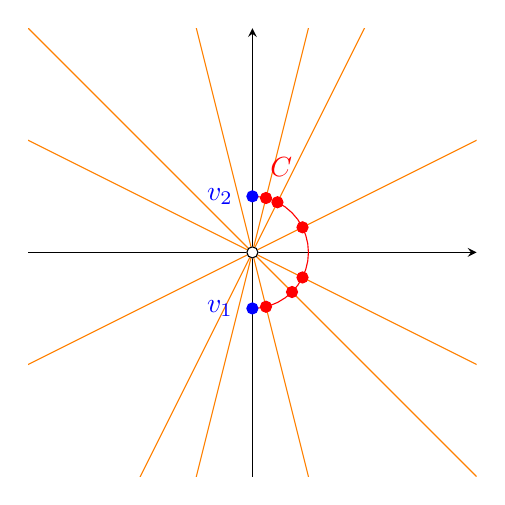
\begin{tikzpicture}
		\begin{axis}[axis equal image,
		axis lines=center,
		ticks=none,
		ymin=-4,ymax=4,
		xmin=-4,xmax=4]
		
			\addplot[color=orange] {2*x};
			\addplot[mark=*,color=red] coordinates {(0.447214,0.894428)};
			\addplot[color=orange] {0.5*x};
			\addplot[mark=*,color=red] coordinates {(0.894427,0.4472135)};
			\addplot[color=orange] {4*x};
			\addplot[mark=*,color=red] coordinates {(0.242536,0.970144)};
			\addplot[color=orange] {-4*x};
			\addplot[mark=*,color=red] coordinates {(0.242536,-0.970144)};
			\addplot[color=orange] {-1*x};
			\addplot[mark=*,color=red] coordinates {(0.707107,-0.707107)};
			\addplot[color=orange] {-0.5*x};
			\addplot[mark=*,color=red] coordinates {(0.894427,-0.4472135)};
			
			\addplot[mark=*,color=blue] coordinates {(0,-1)}
				node[label=left:$v_1$]{};
			\addplot[mark=*,color=blue] coordinates {(0,1)}
				node[label=left:$v_2$]{};
			
			\addplot[mark=*,color=white] coordinates {(0,0)};
			\addplot[mark=o] coordinates {(0,0)};
			
			
			\addplot [domain=-90:90, samples=21, color=red] ({cos(x)},{sin(x)})
				node[label=50:$C$]{};
		\end{axis}
		\end{tikzpicture}
		\end{center}
		Pero el problema ahora viene por que $v_1$ y $v_2$ corresponden al mismo elemento de
		$\Po^1_\real$. Lo podemos solucionar de la siguiente forma:
		\begin{center}
		\begin{tikzpicture}
		\begin{axis}[
			axis lines=center,
			axis equal,
			hide axis,
			enlargelimits=0.1
		]
			\addplot [domain=-180:180, samples=50, color=red] ({cos(x)},{sin(x)});
			
			\addplot [mark=*,color=blue] coordinates {(-1,0)}
				node[label=left:$\infty$]{};
		\end{axis}
		\end{tikzpicture}
		\end{center}
		De tal forma que 
		\[
			\bb{A}^1_\real \cup \setb{\infty} = \Po^1_\real = C/(v_1 \sim v_2)
		\]
		\item $\Po^2_{\real}$.
		\begin{center}
		\begin{tikzpicture}
		\begin{axis}[%
		axis equal,
		ticks=none,
		width=\columnwidth,
		enlargelimits=0,
		axis lines=center,
		view={10}{20},
		ymin=-4,ymax=4,
		xmin=-4,xmax=4
		]
		
			\draw [color=orange] (axis cs:-4,-4,-4) -- (axis cs:4,4,4);
			\addplot3 [mark=*,color=red] coordinates {(1,1,1)};
			\draw [color=orange] (axis cs:4,-2,-4) -- (axis cs:-4,2,4);
			\addplot3 [mark=*,color=red] coordinates {(1,-0.5,-1)};
			\draw [color=orange] (axis cs:-4,-2,0) -- (axis cs:4,2,0);
			\addplot3 [mark=*,color=red] coordinates {(1,0.5,0)};
			\draw [color=orange] (axis cs:-4,8,-12) -- (axis cs:4,-8,12);
			\addplot3 [mark=*,color=red] coordinates {(1,-2,3)};
			
			\addplot3[mark=*,color=white] coordinates {(0,0,0)};
			\addplot3[mark=o] coordinates {(0,0,0)};
			
			\addplot3 [patch, patch type=rectangle,opacity=.5,color=red]
			coordinates { (1,4,4) (1,-4,4) (1,-4,-4) (1,4,-4) }
			node[pin={[black]right:$\bb{A}^2_\real$}]{};
		\end{axis}
		\end{tikzpicture}
		\end{center}
		Cada objeto de $\Po^2_\real$ (rectas en naranja) tiene su equivalente en
		$\bb{A}^2_\real$ (puntos en rojo), a excepción de las rectas del plano $x=0$.
		Para solucionar este problema, procedemos de manera análoga a \ref{item:po1r}
		\begin{center}
		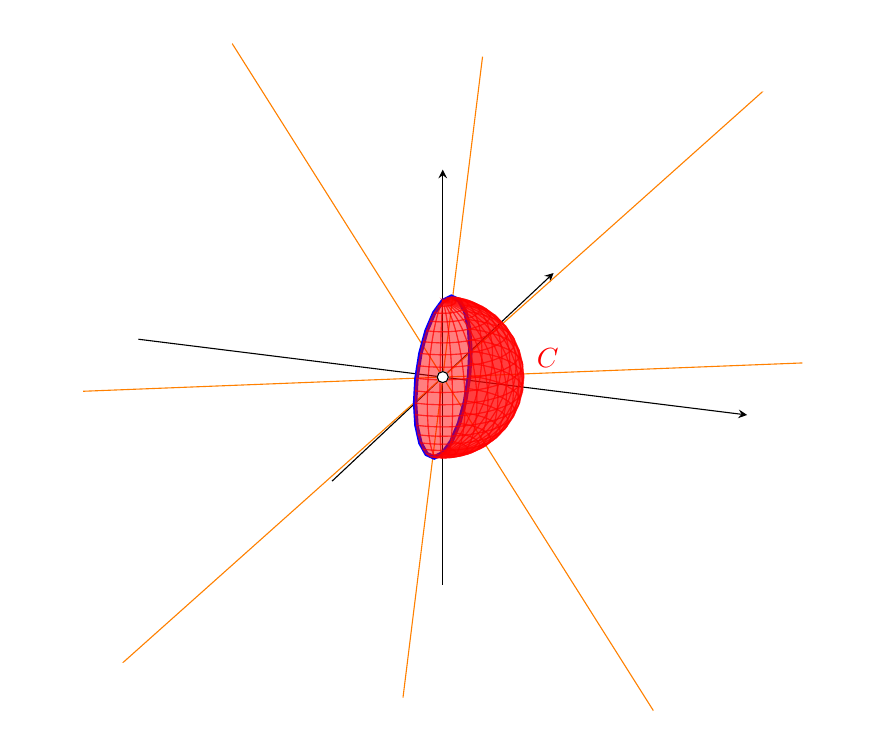
\begin{tikzpicture}
		\begin{axis}[%
		axis equal,
		ticks=none,
		width=\columnwidth,
		enlargelimits=0,
		axis lines=center,
		view={20}{20},
		ymin=-4,ymax=4,
		xmin=-4,xmax=4
		]
			\draw [color=orange] (axis cs:-4,-4,-4) -- (axis cs:4,4,4);
			\draw [color=orange] (axis cs:4,-2,-4) -- (axis cs:-4,2,4);
			\draw [color=orange] (axis cs:-4,-2,0) -- (axis cs:4,2,0);
			\draw [color=orange] (axis cs:-4,8,-12) -- (axis cs:4,-8,12);
			
			\addplot3[mark=*,color=white] coordinates {(0,0,0)};
			\addplot3[mark=o] coordinates {(0,0,0)};
			
			\addplot3[
			color=blue,
			samples=21,
			variable = \v,
			domain = 0:360,
			ultra thick
			]
			({0},{cos(v)},{sin(v)});
			
			\addplot3[%
			opacity = 0.5,
			surf,
			color=red,
			faceted color=red,
			z buffer = sort,
			samples = 21,
			variable = \u,
			variable y = \v,
			domain = -90:90,
			y domain = 0:180,
			]
			({cos(u)*sin(v)}, {sin(u)*sin(v)}, {cos(v)});
			
			\addplot3 [mark=none,color=red] coordinates {(1,0,0)}
				node[label=50:$C$]{};
		\end{axis}
		\end{tikzpicture}
		\end{center}
		De nuevo, nos encontramos con el problema de que hay elementos de $C$ (en azul)
		que se corresponden con el mismo elemento de $\Po^2_\real$, No obstante, podemos
		visualizarlo como
		\begin{center}
		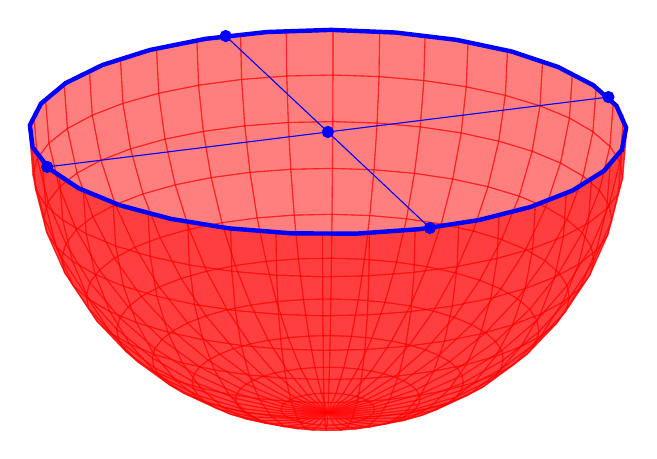
\begin{tikzpicture}
		\begin{axis}[axis equal,
		ticks=none,
		width=\columnwidth,
		enlargelimits=0,
		axis lines=center,
		hide axis,
		view={10}{20},
		ymin=-1.2,ymax=1.2,
		xmin=-1.2,xmax=1.2
		]
			\addplot3[%
			opacity = 0.5,
			surf,
			color=red,
			faceted color=red,
			z buffer = sort,
			samples = 21,
			variable = \u,
			variable y = \v,
			domain = 0:180,
			y domain = 90:270,
			]
			({cos(u)*sin(v)}, {sin(u)*sin(v)}, {cos(v)});
			
			\addplot3[
			color=blue,
			samples=30,
			variable = \v,
			domain = 0:360,
			ultra thick
			]
			({cos(v)},{sin(v)},{0});
			
			\addplot3 [mark=*,color=blue] coordinates {(0,0,0)};
			\addplot3 [mark=*,color=blue] coordinates {({cos(30)},{sin(30)},0)};
			\addplot3 [mark=*,color=blue] coordinates {({cos(210)},{sin(210)},0)};
			\draw (axis cs: {cos(30)}, {sin(30)}, 0) [color=blue] --
				(axis cs: {cos(210)}, {sin(210)}, 0);
				
			\addplot3 [mark=*,color=blue] coordinates {({cos(120)},{sin(120)},0)};
			\addplot3 [mark=*,color=blue] coordinates {({cos(300)},{sin(300)},0)};
			\draw (axis cs: {cos(120)}, {sin(120)}, 0) [color=blue] --
				(axis cs: {cos(300)}, {sin(300)}, 0);
			
			
		\end{axis}
		\end{tikzpicture}
		\end{center}
		Y unir los puntos azules antipolares. Aunque, si lo tratamos de imaginar, este
		objeto, no cabe en $\real^3$.
		\item $\Po^1_{\cx} = (\cx^2 \setminus {0})/\sim \ = \cx \cup \setb{\infty} = S^2$. Las igualdades por el momento son
        por analogía o intuición, más adelante se demostrarán. Aunque nos podemos hacer una idea basandonos en la proyección
        estereográfica
		\begin{center}
		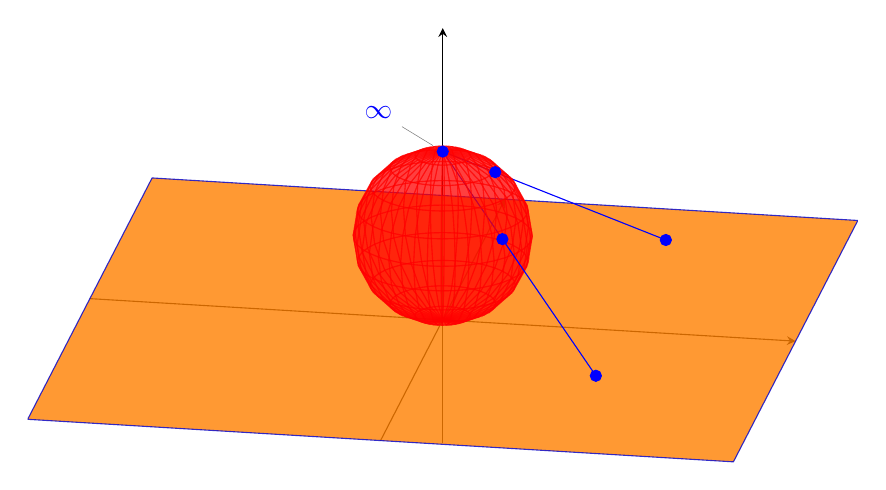
\begin{tikzpicture}
		\begin{axis}[axis equal,
		ticks=none,
		width=\columnwidth,
		enlargelimits=0,
		axis lines=center,
		view={10}{20},
		ymin=-4,ymax=4,
		xmin=-4,xmax=4]
		
			\addplot3[patch,color=orange, patch type=rectangle, opacity=0.8] coordinates
			{(4,4,0) (4,-4,0) (-4,-4,0) (-4,4,0)};
		
			\addplot3[color=blue,mark=*] coordinates {(0,0,2)} node[pin=150:{$\infty$}]{};
			
			\addplot3[mark=*,color=blue] coordinates {(2,3,0)};
			\addplot3[mark=*,color=blue] coordinates {(0.47,0.71,1.53)};
			\draw (axis cs:0,0,2) [color=blue] -- (axis cs:2,3,0);
			
			\addplot3[mark=*,color=blue] coordinates {(2,-1.5,0)};
			\addplot3[mark=*,color=blue] coordinates {(0.78,-0.59,1.22)};
			\draw (axis cs:0,0,2) [color=blue] -- (axis cs:0.78,-0.59,1.22);
			
			\addplot3[%
			opacity = 0.5,
			surf,
			color=red,
			faceted color=red,
			z buffer = sort,
			samples = 21,
			variable = \u,
			variable y = \v,
			domain = 0:180,
			y domain = 0:360,
			]
			({cos(u)*sin(v)}, {sin(u)*sin(v)}, {cos(v)+1});
	
			\draw (axis cs:0.78,-0.59,1.22)[color=blue] -- (axis cs:2,-1.5,0);
			
		\end{axis}
		\end{tikzpicture}
		\end{center}
		
		\item $\Po^2_{\z / 2}$ contiene $7$ puntos pues las rectas de $\z^3$ solo contienen el $0$ y un punto.
	\end{enumerate}
\end{example}
\begin{obs}
	Hemos enunciado la definición algebraica de $\Po_{\real}^{n}$. Existe una definición axiomática que no 
	es igual en algunos casos patológicos.
\end{obs}

\subsection{Variedades lineales proyectivas}

\begin{defi}
	Sea $\E$ un $\k$-e.v. de dimensión $n+1$, sea $\Po^n = \Po(\E)$.
	Llamaremos variedad lineal (proyectiva) de dimensión $r$ a cualquier conjunto 
	de la forma:
	\[V = \pi(H \setminus \setb{0})\]
	donde $H \subseteq \E$ es un subespacio vectorial de dimensión $r+1$.
	
	Por convención defnimos la siguiente notación:
	\[V = \pi(H \setminus \setb{0}) = \pi(H)\]         
\end{defi}    
\begin{example}
	\begin{itemize}
		\item []
		\item $\Po^n = \pi(\E)$ es una variedad lineal de dimensión $n$.
		\item $p \in \Po^n$, $p = \pi(v) = \pi([v])$ es una varidead lineal de dimensión $0$.
		\item $\emptyset = \pi({\emptyset_{\E}})$ es una variedad lineal de dimensión $-1$.
	\end{itemize}
\end{example}
\begin{defi}
	\begin{itemize}
		\item []
		\item $\dim V = 1 \longrightarrow$ Recta
		\item $\dim V = 2 \longrightarrow$ Plano
		\item $\dim V = n-1 \longrightarrow$ Hiperplano
	\end{itemize}
\end{defi}
\begin{lema}
	$V = \pi(H\setminus\setb{0}) \iff H \setminus \setb{0} = \pi^{-1}(V)$
\end{lema}
\begin{ej}
	Demostrar el lema anterior.
\end{ej}
\begin{obs}
	Hay una biyección
	\[\setb{\text{s.e.v. de } \E}
	\mathrel{\mathop{\rightleftarrows}^{\mathrm{\pi}}_{\mathrm{\pi^{-1}}}}
	\setb{\text{variedades lineales de } \Po(\E)}\]
	\begin{itemize}
		\item con dimension $r+1 \leftrightarrow r$
		\item $H_1 \subseteq H_2 \iff V_1 \subseteq V_2$ con $V_i=\pi(H_i)$
		\item Las operaciones $+$ y $\cap$ definidas para subespacios, se definen
		a traves de esta biyección a variedades.
	\end{itemize}
\end{obs}
\begin{prop}
    Sean $V_1, V_2 \subseteq \Po^n$ variedades lineales $\implies V_1 \cap V_2$ variedad lineal que verifica:
    \begin{itemize}
        \item $V_1 \cap V_2 \subseteq V_1, V_2$
        \item Si $W$ variedad lineal, $W \subseteq V_1, V_2$ i $W \subseteq V_1 \cap V_2$
    \end{itemize}
\end{prop}
\begin{proof}
    Veamos que: $V_1 \cap V_2 = \pi(H_1 \cap H_2)$ si $V_i = \pi(H_i)$ \\
    $\supseteq$
    \begin{gather*} 
    \text{Si } v \in H_1 \cap H_2, p = [v] \in \pi(H_1), \pi(H_2) \implies p \in V_1 \cap V_2
    \end{gather*}
    $\subseteq$
    \begin{gather*}
        \text{Sea } p \in V_1 \cap V_2,
        \begin{rcases} p = [v_1], v_1 \in H_1 \\ p = [v_2], v_2 \in H_2 \end{rcases} \implies [v_1] = [v_2] \implies
        \exists \lambda \neq 0 \text{ t.q. } v_2 = \lambda v_1 \implies \\ \implies v_2 \in H_1 \implies v_2 \in H_1
        \cap H_2 \implies p = [v_2] \in \pi (H_1 \cap H_2)
    \end{gather*}
    El resto sigue de lo que sabemos de s.e.v.s.
\end{proof}
\begin{defi}
    Sean $V_1, V_2 \subseteq \Po^n$ variedades lineales, $V_i = \pi (H_i)$, definimos \textit{join} o variedad lineal generada como:
    \[
    V_1 \vee V_2 = \pi (H_1 + H_2)
    \]
\end{defi}
\begin{prop}
    \begin{itemize}
    \item[]
    \item $V_1, V_2 \subseteq V_1 \vee V_2$
    \item Sea $W$ una variedad lineal, $V_1, V_2 \subseteq W \implies V_1 \vee V_2 \subseteq W$
    \end{itemize}
\end{prop}
\begin{proof}
    Propiedades de la suma de s.e.v.
\end{proof}
\begin{prop}
    Sean $V_1, V_2 \subseteq \Po^n$ variedades lineales:
    \begin{itemize}
        \item $V_1 \subseteq V_2 \implies \dim \left( V_1\right) \leq \dim \left( V_2 \right)$
        \item Si $V_1 \subseteq V_2$ y $\dim \left( V_1 \right) = \dim \left( V_2 \right) \implies V_1 = V_2$
    \end{itemize}
\end{prop}
\begin{prop}[Fórmula de Grassmann]
    \[ \dim \left( V_1 \cap V_2 \right) + \dim \left( V_1 \vee V_2 \right) = \dim \left( V_1 \right) + \dim \left( V_2 \right) \]
\end{prop}
\begin{proof}
    Propiedades s.e.v.
\end{proof}
\begin{example}
    \begin{enumerate}
        \item[]
        \item $\Po^2 \quad V_1, V_2$ rectas, tenemos que $\dim \left( V_1 \cap V_2 \right) + \dim \left( V_1 \vee V_2 \right) = 2$ (Grassmann).
        \begin{center} \begin{tabular}{|c|c|c|}
            \hline $\dim \left( V_1 \cap V_2 \right)$ & $1 \leq \dim \left( V_1 \vee V_2 \right) \leq 2$  & Posición relativa \\
            \hline \hline
            0 & 2 & Se cortan en un punto \\ \hline
            1 & 1 & Son la misma recta\\ \hline
        \end{tabular} \end{center}
        Por tanto, dos rectas en un plano, o se cruzan o son la misma.
        \item $\Po^3 \quad V_1, V_2$ rectas, tenemos que $\dim \left( V_1 \cap V_2 \right) + \dim \left( V_1 \vee V_2 \right) = 2$ (Grassmann).
        \begin{center} \begin{tabular}{|c|c|c|}
            \hline $\dim \left( V_1 \cap V_2 \right)$ & $1 \leq \dim \left( V_1 \vee V_2 \right) \leq 3$  & Posición relativa \\
            \hline \hline
            -1 & 3 & Se cruzan \\ \hline
            0 & 2 & Se cortan en un punto $\left( V_1 \vee V_2 \cong \Po^2 \right)$ \\ \hline
            1 & 1 & Son la misma recta\\ \hline
        \end{tabular} \end{center}
        \item $\Po^3 \quad V_1, V_2$ planos, tenemos que $\dim \left( V_1 \cap V_2 \right) + \dim \left( V_1 \vee V_2 \right) = 4$ (Grassmann).
        \begin{center} \begin{tabular}{|c|c|c|}
            \hline $\dim \left( V_1 \cap V_2 \right)$ & $2 \leq \dim \left( V_1 \vee V_2 \right) \leq 3$  & Posición relativa \\
            \hline \hline
            1 & 3 & Se cortan en una recta \\ \hline
            2 & 2 & Son el mismo plano\\ \hline
        \end{tabular} \end{center}
        \item $\Po^3 \quad V_1$ plano, $V_2$ recta, tenemos que $\dim \left( V_1 \cap V_2 \right) + \dim \left( V_1 \vee V_2 \right) = 3$ (Grassmann).
        \begin{center} \begin{tabular}{|c|c|c|}
            \hline $\dim \left( V_1 \cap V_2 \right)$ & $2 \leq \dim \left( V_1 \vee V_2 \right) \leq 3$  & Posición relativa \\
            \hline \hline
            0 & 3 & Se cortan en un punto \\ \hline
            1 & 2 & $V_2 \subseteq V_1$ \\ \hline
        \end{tabular} \end{center}
    \end{enumerate}
\end{example}
\begin{prop}
    Sean $p \in \Po^n, r, V, H \subseteq \Po^n$ (recta, variedad lineal, hiperplano, respectivamente).
    \begin{enumerate}
        \item $\dim \left( V \vee p \right) = \text{ ó } \begin{cases} \dim V & (\iff p \in V) \\ \dim V + 1 & (\iff p \notin V) \end{cases}$
        \item $\dim \left( r \vee H \right) = \text{ ó } \begin{cases} 1 & (\iff r \subseteq H) \\ 0 & (\iff r \nsubseteq H) \end{cases}$
    \end{enumerate}
\end{prop}
\begin{proof}
    Fórmula de Grassmann.
\end{proof}
\begin{defi}
    Sean $V_1, V_2 \subseteq \Po^n, (V_i = \pi \left( H_i \right)$ variedades lineales, $V_1$ y $V_2$ son suplementarias $\iff H_1$ y $H_2$
    son complementarios.
\end{defi}
\begin{obs}
    $V_1, V_2$ suplementarias $\iff H_1 \oplus H_2 = \E \iff \left. \begin{cases} (1) & H_1 + H_2 = \E \\ (2) & H_1 \cap H_2 \end{cases} \right\}
    \iff \begin{cases} (1) & V_1 \vee V_2 = \Po^n \\ (2) & V_1 \cap V_2 = \emptyset \end{cases}$
\end{obs}
\begin{prop}
    Sean $V_1, V_2 \subseteq \Po^n$ variedades lineales:
    \begin{enumerate}
        \item $V_1, V_2$ son suplementarias $\implies \dim V_1 + \dim V_2 = n-1$
        \item Si $\dim V_1 + \dim V_2 = n-1$
        \[
        V_1, V_2 \text{ suplementarias} \iff V_1 \vee V_2 = \Po^n \iff V_1 \cap V_2 = \emptyset
        \]
    \end{enumerate}
\end{prop}
\begin{proof}
    \begin{enumerate}
        \item[]
        \item $V_1, V_2$ suplementarias $\iff H_1, H_2$ complementarios $\implies \overbrace{\dim H_1}^{\dim V_1 + 1} +
        \overbrace{\dim H_2}^{\dim V_2 + 1} = \dim \E = n+1$
        \item Fórmula de Grassmann.
    \end{enumerate}
\end{proof}
\begin{defi}
    Sea $\Po^n = \real(\E )$, y sean $p_0, \dots, p_m \in \Po^n$ tal que $p_i = [v_i], v_i \in \E$, decimos que $p_0, \dots,
    p_m$ son linealmente independientes (l.i.) $\iff v_1, \dots, v_m \in \E$ son linealmente independientes.
\end{defi}
\begin{obs}
    La independencia lineal no depende de los representantes elegidos.
\end{obs}
\begin{example}
    $\Po^2_\real = \Po(\real^3)$. Sean $p_0 = [(1,1,0)], p_1 = [(0,1,1)], p_2 = [(2,3,1)]$. Entonces $p_0$ y $p_1$ son l.i.,
    pero $p_0, p_1, p_2$ son l.d..
\end{example}
\begin{prop}
    Sean $p_0, \dots, p_m \in \Po^n$ puntos y $V \subseteq \Po^n$ una variedad lineal:
    \begin{enumerate}
        \item $\dim\left( p_0 \vee \dots \vee p_m \right) \leq m$
        \item $\dim\left( p_0 \vee \dots \vee p_m \right) = m \iff p_0, \dots, p_m$ son l.i.
        \item $\dim V = m \iff \exists p_0, \dots, p_m \in V$ tal que $V = p_0 \vee \dots \vee p_m
            \iff \forall p_0, \dots, p_m \in V \text{ l.i.}, V = p_0 \vee \dots \vee p_m$
    \end{enumerate}
\end{prop}
\begin{proof}
    Inmediata a partir de propiedades de s.e.v..
\end{proof}
\begin{defi}
    $p_0, \dots, p_r \in \Po^n (r \geq n)$ estan en posición general $\iff n+1$ puntos cualesquiera de ellos son l.i..
\end{defi}

\subsection{Sistemas de referencia proyectivos. Coordenadas proyectivas}

\begin{obs}
    $\Po^n = \Po(\E)$. Sea $B = \{v_0, \dots, v_n\}$ base de $\E$:
    \begin{center} \begin{tabular}{ccc}
        $p = [v] = [\lambda v] \qquad $ &
        $(v)_B = \begin{pmatrix} x_0 \\ \vdots \\ x_n \end{pmatrix}\qquad $&
        $(\lambda v)_B = \begin{pmatrix} \lambda x_0 \\ \vdots \\ \lambda x_n \end{pmatrix} \qquad$
    \end{tabular} \end{center}
    Vemos que las coordenadas estarían definidas salvor por multiplicar por $\lambda$.
\end{obs}
\begin{defi}
    $\Po^n = \Po(\E)$
    \begin{enumerate}
        \item Un sistema de referencia proyectivo en $\Po^n$ es:
            \[ R= \{ p_0, \dots, p_n; \bar{p} \} \]
            Donde $p_0, \dots, p_n, \bar{p}$ estan en posición general.
            \begin{itemize}
                \item $\{ p_0, \dots, p_n \}$ son los vertices de $R$
                \item $\bar{p}$ es el punto unidad
            \end{itemize}
        \item Fijado un sistema de referencia $R$. Sea $B = \{ u_0, \dots, u_n \}$ base de $\E$. Diremos que $B$ esta adaptada a $R$ si y solo si:
            \[ \begin{cases} p_i = [u_i], \forall i = 0, \dots, n \\ \bar{p} = [u_0 + \dots + u_n ] \end{cases} \]
        \item \textit{Asignación de coordenadas proyectivas} \\
            $\Po^n = \Po(\E)$, Sea $R = \{ p_0, \dots, p_n; \bar{p} \}$, y $B = \{u_0, \dots, u_n\}$ una base adaptada. Sea $q \in \Po^n, q = [v]$, entonces 
            $q_R = v_B$. (Cale ver que la definición es consistente)
    \end{enumerate}
\end{defi}
\begin{prop}
    Sea $R$ un sistema de referencia en $\Po^n$. Sean $B_1 = \{ u_0, \dots, u_n\}, B_2 = \{ u'_0, \dots u'_n \}$ bases adaptadas a $R$. Sea $q = [v] \in \Po^n$, entonces $\exists \lambda \neq 0$ tal que $v_{B_2} = v_{B_1}$.
\end{prop}
\begin{proof}
    $p_i = [u_i] = [u'_i], \forall i = 0, \dots, n$. Por tanto, $\exists \lambda \neq 0$ tal que $u'i= \lambda_i u_i, \forall i = 1, \dots, n$. Por otro lado,
    \begin{gather*}
        \bar{p} = [u_0 + \dots + u_n] = [u'_0 + \dots + u'_n] \implies \exists \lambda \neq 0 \text{ tal que } u'_0 + \dots + u'_n = \\ = \lambda_0 u_0 + \dots + \lambda_n u_n = \lambda (u_0 + \dots + u_n)
        \stackrel{B_1 \text{ base}}{\implies} \lambda_i = \lambda \forall i = 1, \dots, n
    \end{gather*}
\end{proof}
\begin{obs}
    $R = \{ p_0, \dots, p_n; \bar{p} \}$ en $\Po^n$
    \begin{enumerate}
        \item $q \in \Po^n, q_R = (a_0, \dots, a_n) = \lambda (a_0, \dots, a_n) \stackrel{\text{notación}}{=} (a_0 : \dots : a_n) \forall \lambda \neq 0$
        \item Ejemplos: \\ $\begin{aligned} (p_0&)_R = (1:0:\dots:0) \\ \vdots& \\ (p_n&)_R = (0:\dots:0:1) \end{aligned}$
        \item $q_R = (0: \dots : 0)$ no existe.
        \item Sea $\Po^2_\real = \Po(\real^3), R = \{ p_0, p_1, p_2; \bar{p} \} = \left\{ [(1,1,0)], [(1,0,1)], [(0,1,1)]; [(3,3,2)]\right\}$, entonces $B = \left\{ [(1,1,0)], [(1,0,1)], [(0,1,1)] \right\}$ no es una base
            adaptada, para que lo sea, debemos multiplicar $v_0, v_1, v_2$ por $\lambda_0, \lambda_1, \lambda_2$ tales que $\bar{p} = \lambda_0 p_0 + \lambda_1 p_1 + \lambda_2 p_2$. En este caso:
            \[
                \begin{cases} \lambda_0 + \lambda_1 = 3 \\ \lambda_0 + \lambda_2 = 3 \\ \lambda_1 + \lambda_2 = 2 \end{cases} \iff \begin{cases} \lambda_0 = 2 \\ \lambda_1 = 1 \\ \lambda_2 = 1 \end{cases}
            \]
            Y el sistema de referencia con la base $B$ adaptada es: \[ R' = \left\{ [(2,2,0)], [(1,0,1)], [(0,1,1)]; [(3,3,2)]\right\} \]
    \end{enumerate}
\end{obs}









